\documentclass{article}

\usepackage[utf8]{inputenc}
\usepackage{CJKutf8}
\usepackage{amsmath}
\usepackage{amsfonts}
\usepackage{url}
%\usepackage{ffcode}
\usepackage{graphicx}

\begin{document}

\begin{CJK}{UTF8}{gbsn}

\section{2022年6月22日}

重复使用feature selection技术之后的结果:\url{https://github.com/Zarrathustra/Machine_Learning_LHY/blob/main/Homework_1/ML2022Spring_HW1_001_feature_selection.ipynb}。Private score: 0.95374。

\subsection{batch size}

因为training data的个数从2160个,比较小,所以尝试较小的batch size。

基于上脚本,将batch size从256改成16。此时,loss function在前期下降得比256时候低,但是后期的最低值不如batch size为256。此时,因为batch size太小,导致无法充分利用GPU资源,从而训练时间很长。

再尝试batch size为64。因为之前尝试了Adam,获得了好效果,所以这次实验基于Adam。Private score:0.91444。相比于batch size为256,结果变差了。

之前亦考虑设定Dataloader每个epoch之前都重新shuffle。通过阅读PyTorch的文档可以知道,Dataloader本身就会做这件事。

当前,不需要对batch size进行修改。

\subsection{Adam}

之前也尝试过Adam,但是learning rate使用的和SGD一样的$10^{-5}$。这次改成使用Adam默认的$10^{-3}$。结果有明显的进步。

脚本存放在\url{https://github.com/Zarrathustra/Machine_Learning_LHY/blob/main/Homework_1/ML2022Spring_HW1_001_feature_selection_Adam.ipynb}。

并且,使用Adam的训练速度很快。这样实验可以进行得很迅速。Private score:0.89699。

\subsection{L2 penalty}\label{sec:L2_penalty}

在Adam之中加入weight decay。

设定weight decay为0.1时,结果没有之前好。

设定weight decay为0.01时,结果也没有之前好。

L2 penalty是为了解决overfitting的问题。所以先加深、加宽神经网络,然后再尝试weight decay。加宽神经网络至1024。

设定weight decay为0.1时,training loss和validation loss都升高了。

设定weight decay为0.01时,training loss和validation loss都升高了。

设定weight decay为0.001时。可以看到如下结果。红线为测试结果。
\begin{figure}[htbp]
    \centering
    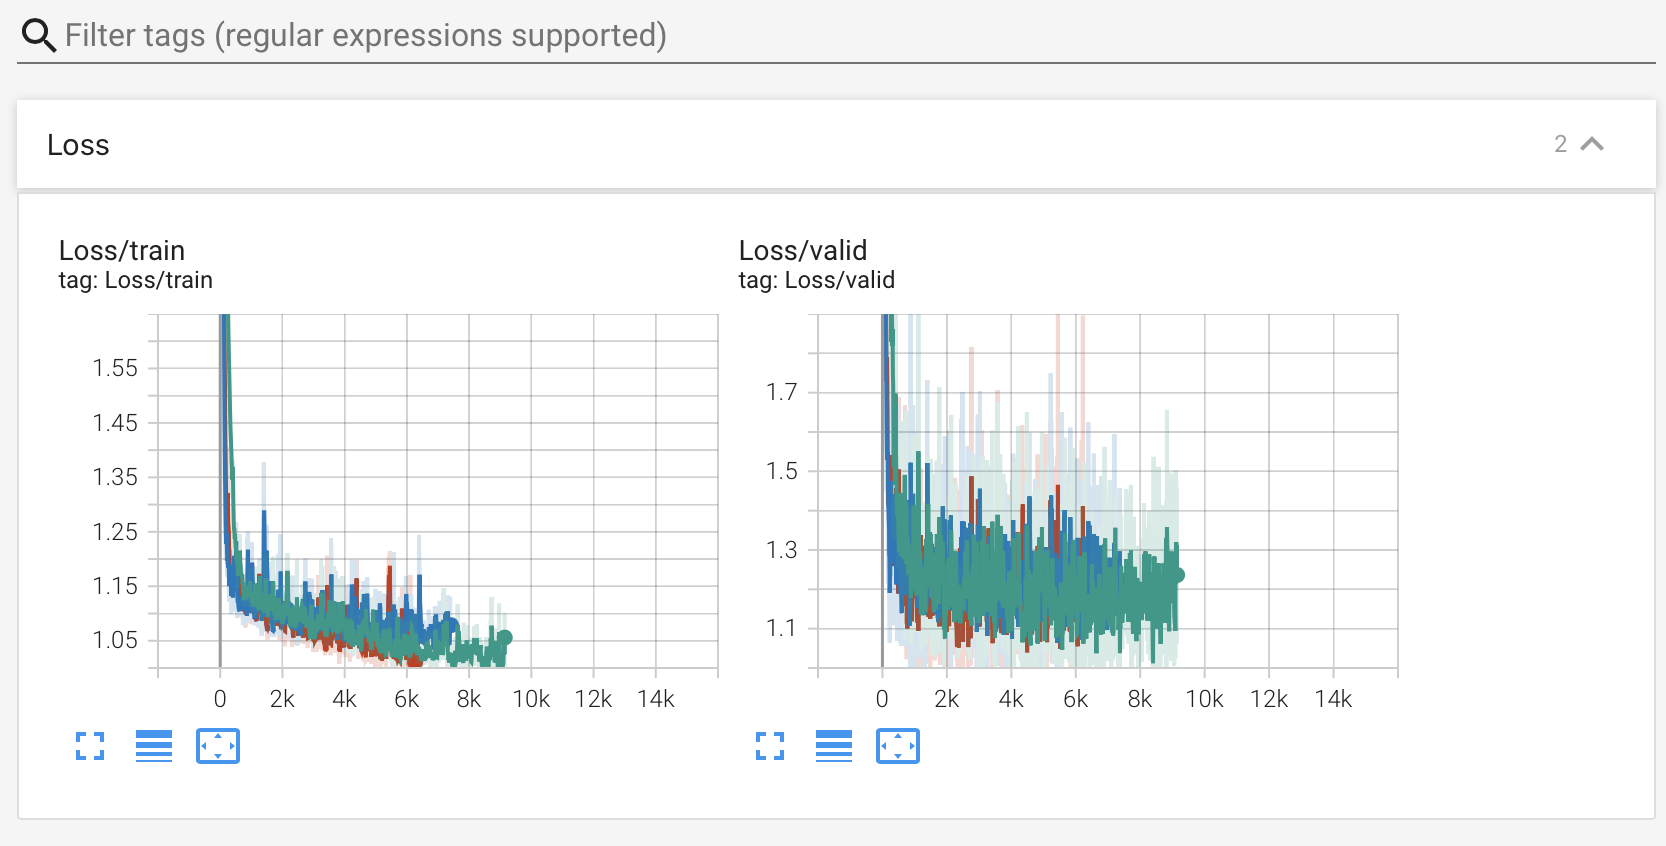
\includegraphics[width=\linewidth]{graphics/FC_1024_weight_decay_0_001.png}
    \caption{加宽神经网络至1024,weight decay为0.001}
    \label{fig:FC_1024_weight_decay_0_001}
\end{figure}
Private score:0.91897。并没有之前高。

先考虑继续加深、加宽神经网络,提高网络在training data上的拟合能力。

加深神经网络,变成了$4096 \rightarrow 512 \rightarrow 64 \rightarrow 8 \rightarrow 1$。

设定weight decay为0.001时,结果不够好。
设定weight decay为0.0001时,结果不够好。Private score:1.02880。说明overfitting了。现在神经网络的拟合能力够了,需要找到更好的解决overfitting的办法。

\subsection{加深、加宽神经网络}

再加入一层$16 \rightarrow 16$的FC神经网络。结果(training loss)没有变好,而且这里最需要注意的是,我们现在关心的是training loss。可以先放任其 overfitting,之后再通过其他的办法解决 overfitting 的问题。 

不再加入一层$16 \rightarrow 16$的FC神经网络。

尝试将原先16宽的神经网络加宽到128。这时候可以明显看到training loss下降了(图\ref{fig:FC_128}),绿线为测试。Private score:0.90486。虽然private score比之前差一点点,但我们现在关心的是training loss。overfitting之后解决。

\begin{figure}[htbp]
    \centering
    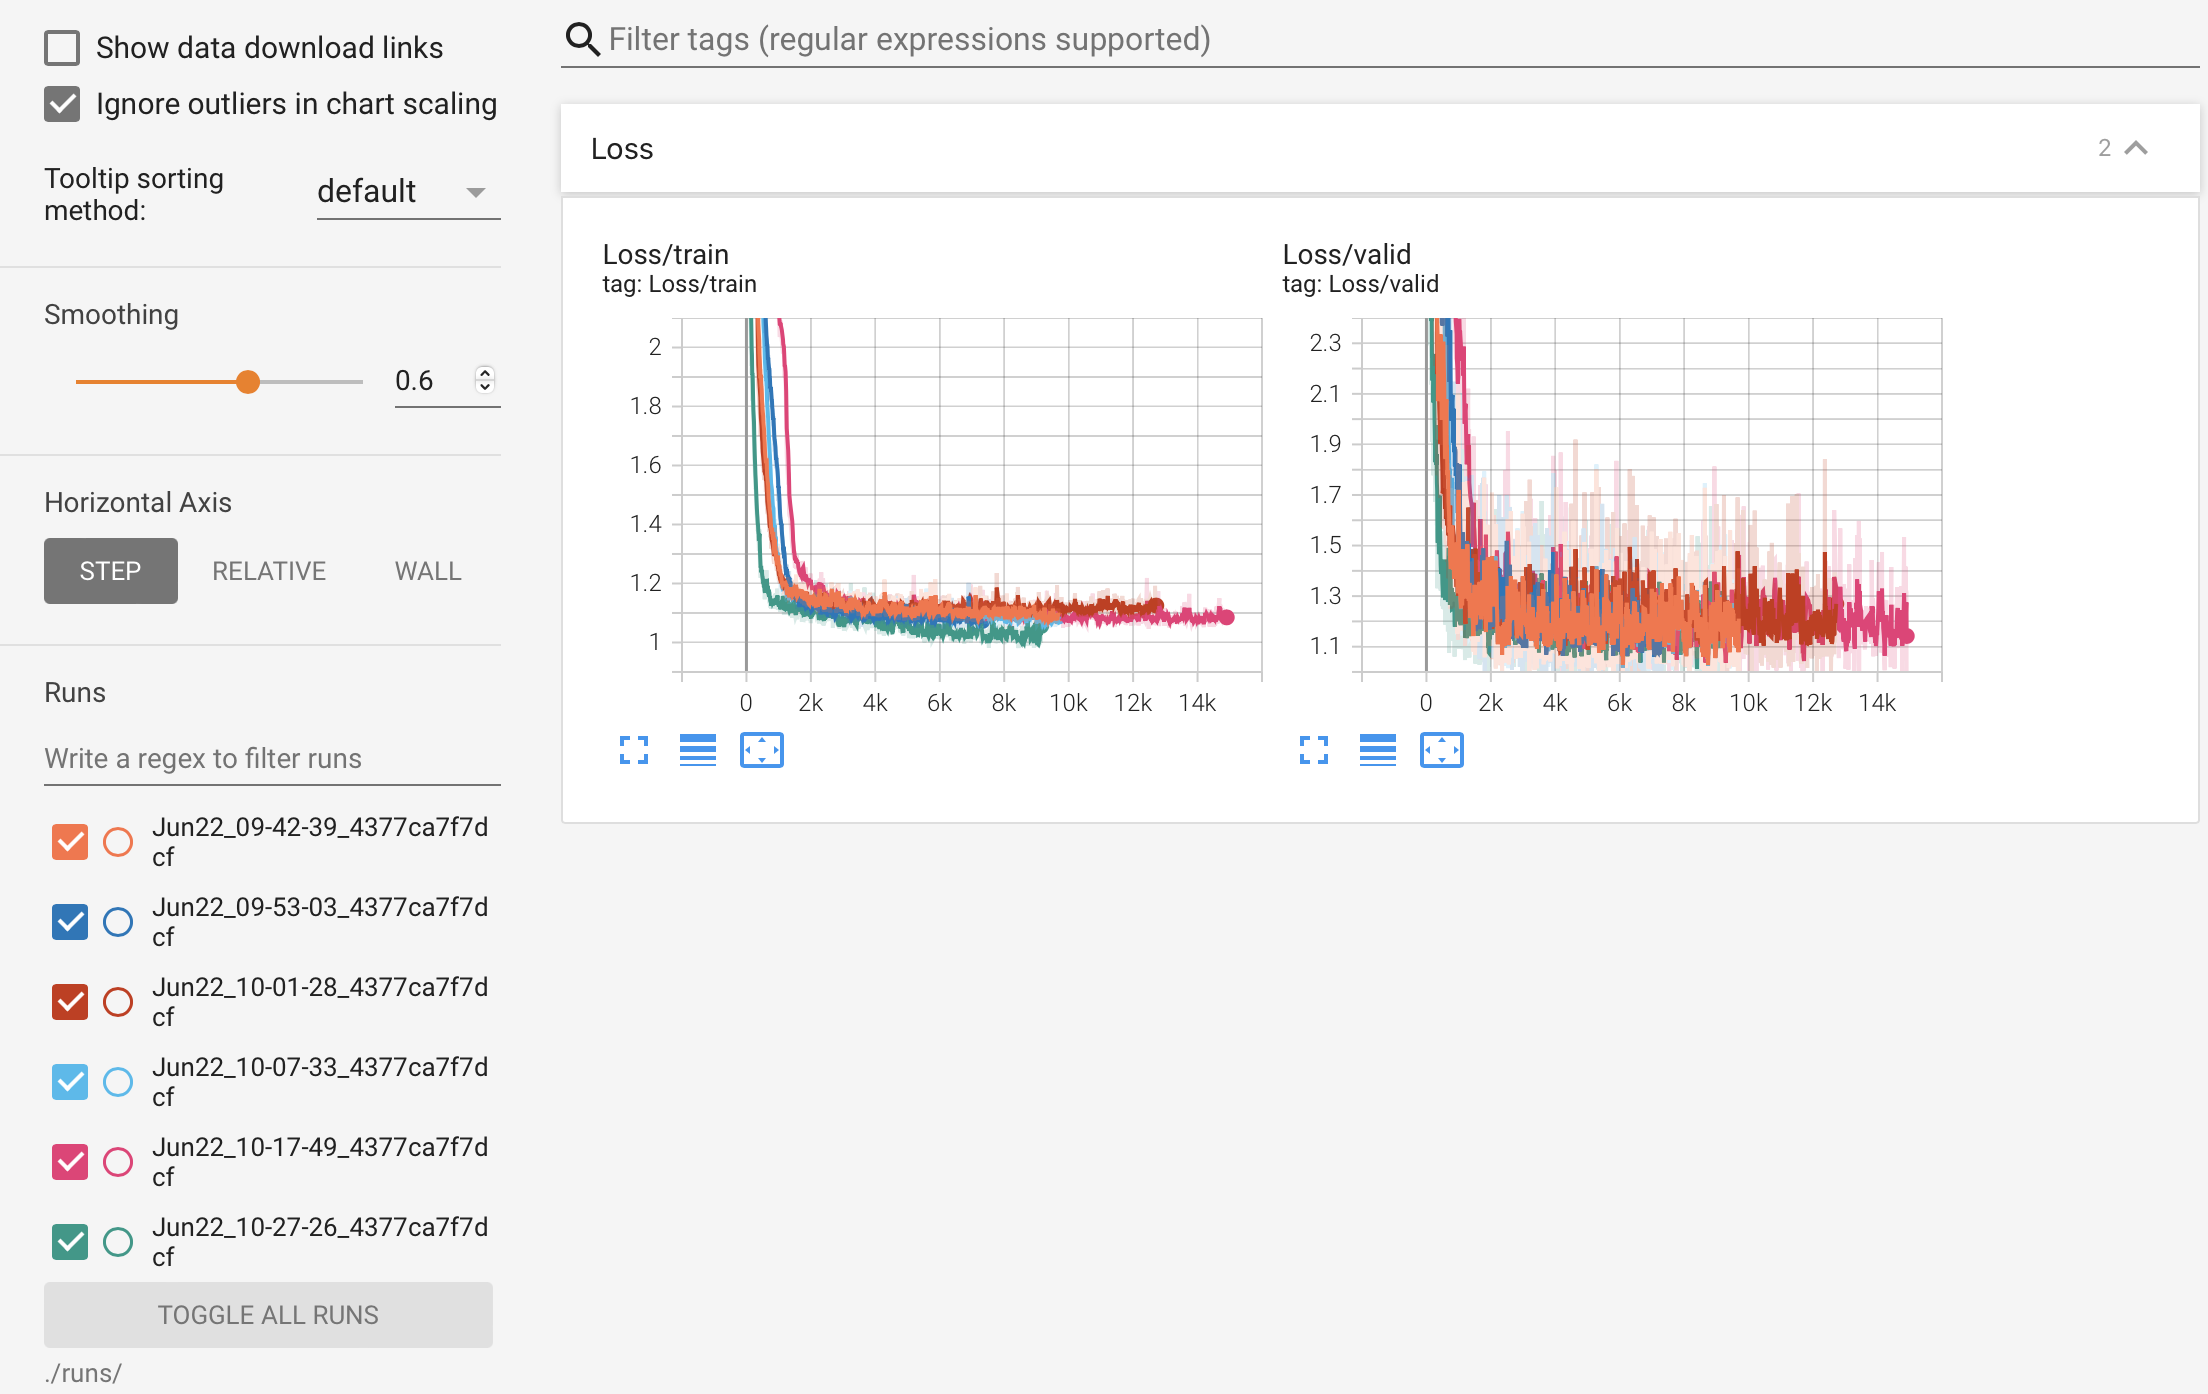
\includegraphics[width=\linewidth]{graphics/FC_128.png}
    \caption{加宽神经网络至128}
    \label{fig:FC_128}
\end{figure}

继续加宽加宽神经网络至1024(图\ref{fig:FC_1024}),灰线为测试。

\begin{figure}[htbp]
    \centering
    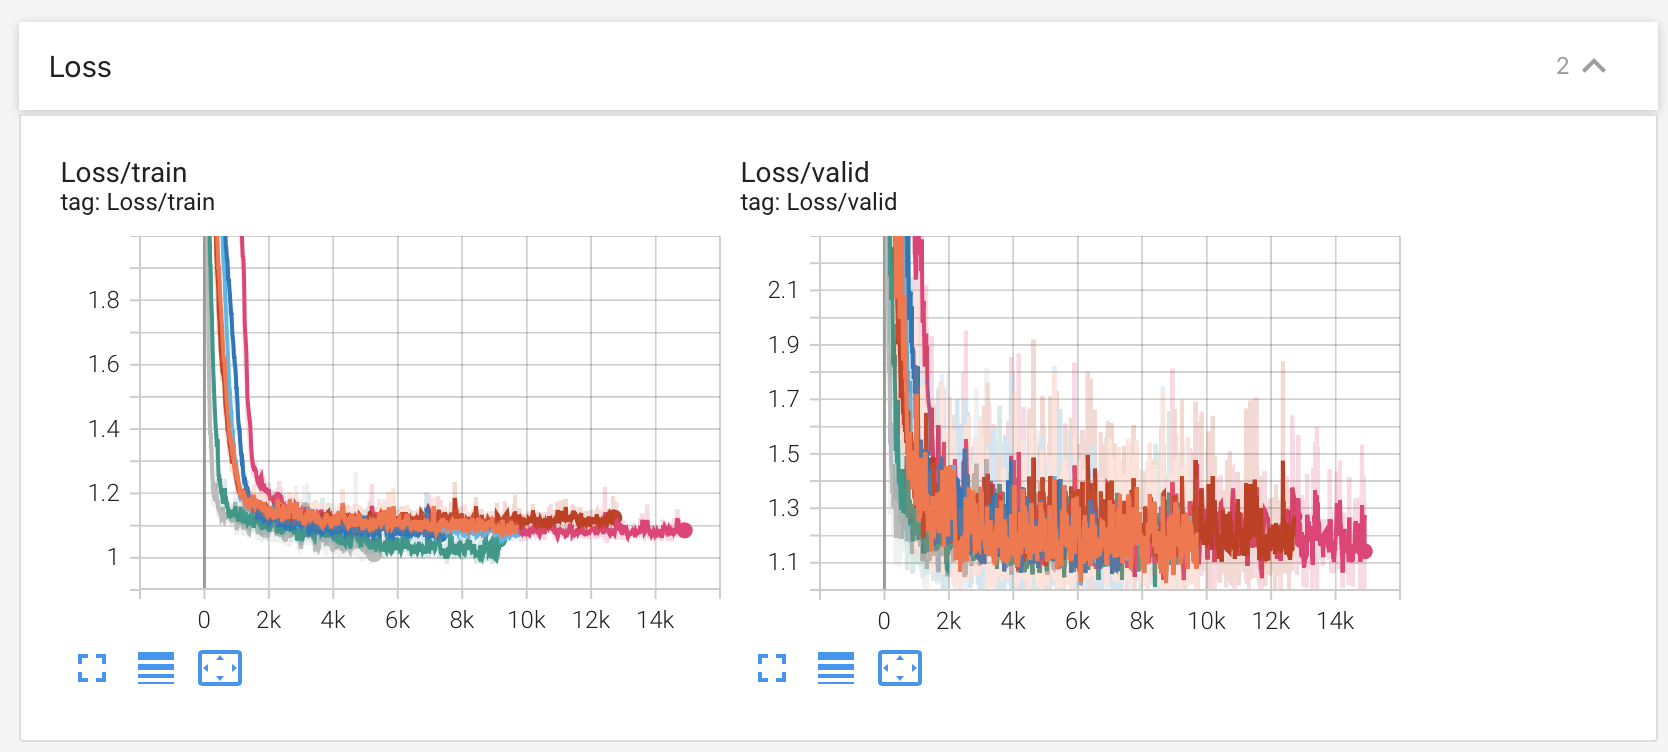
\includegraphics[width=\linewidth]{graphics/FC_1024.png}
    \caption{加宽神经网络至1024}
    \label{fig:FC_1024}
\end{figure}

现在神经网络的表达能力足够了,现在需要去解决overfitting。回到Section \ref{sec:L2_penalty}去解决。

现在发现weight decay加入之后结果不好。

继续增加神经网络的表达能力。增加一层$1024 \rightarrow 256$,此时可以看到training loss继续下降(图\ref{fig:FC_1024_FC_256})。

\begin{figure}[htbp]
    \centering
    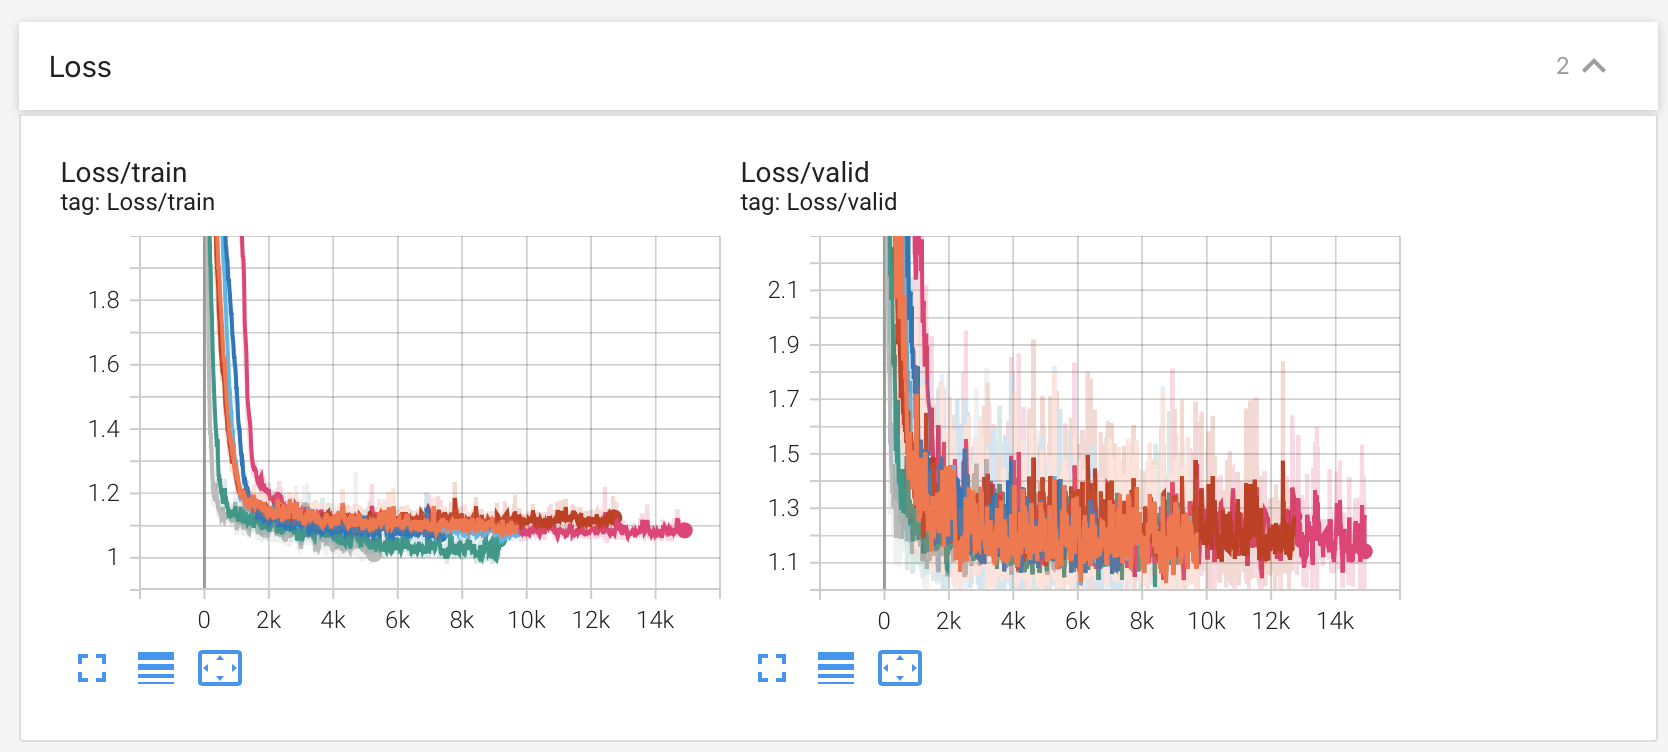
\includegraphics[width=\linewidth]{graphics/FC_1024.png}
    \caption{加宽神经网络至1024}
    \label{fig:FC_1024_FC_256}
\end{figure}

继续增加神经网络的表达能力,变成了$4096 \rightarrow 512 \rightarrow 64 \rightarrow 8 \rightarrow 1$这样一个神经网络。training loss进一步下降。回到Section \ref{sec:L2_penalty}去解决。

\subsection{Dropout}

目前使用L2 penalty没有达到比较好的效果。尝试使用Dropout,也没有明显的效果。

\end{CJK}

\end{document}